% 固定来源PDF印刷页51第2题四个图象选项的矢量示意重绘。
% 渐近线位置、分支象限及选项标签忠于原页；比例仅作示意。
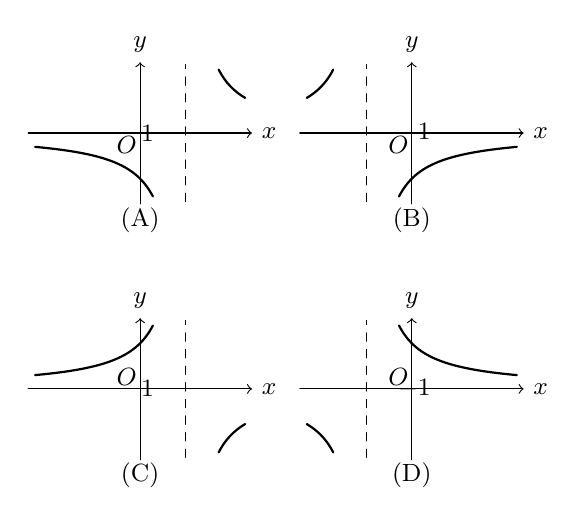
\begin{tikzpicture}[x=.58cm,y=.58cm,font=\small,line cap=round,line join=round]
  % (A) y=1/(x-1)
  \begin{scope}
    \draw[->] (-2.45,0)--(2.45,0) node[right] {$x$};
    \draw[->] (0,-1.55)--(0,1.55) node[above] {$y$};
    \draw[dashed] (1,-1.5)--(1,1.5);
    \draw[thick,domain=-2.3:.28,samples=60,variable=\x] plot (\x,{1/(\x-1)});
    \draw[thick,domain=1.72:2.3,samples=60,variable=\x] plot (\x,{1/(\x-1)});
    \node[left=8pt] at (1,0) {$1$};
    \node[below left,inner sep=1pt] at (0,0) {$O$};
    \node at (0,-1.9) {(A)};
  \end{scope}

  % (B) y=-1/(x+1), the graph of the stated function.
  \begin{scope}[xshift=3.45cm]
    \draw[->] (-2.45,0)--(2.45,0) node[right] {$x$};
    \draw[->] (0,-1.55)--(0,1.55) node[above] {$y$};
    \draw[dashed] (-1,-1.5)--(-1,1.5);
    \draw[thick,domain=-2.3:-1.72,samples=60,variable=\x] plot (\x,{-1/(\x+1)});
    \draw[thick,domain=-.28:2.3,samples=60,variable=\x] plot (\x,{-1/(\x+1)});
    \node[right=8pt] at (-1,0) {$-1$};
    \node[below left,inner sep=1pt] at (0,0) {$O$};
    \node at (0,-1.9) {(B)};
  \end{scope}

  % (C) y=-1/(x-1)
  \begin{scope}[yshift=-3.25cm]
    \draw[->] (-2.45,0)--(2.45,0) node[right] {$x$};
    \draw[->] (0,-1.55)--(0,1.55) node[above] {$y$};
    \draw[dashed] (1,-1.5)--(1,1.5);
    \draw[thick,domain=-2.3:.28,samples=60,variable=\x] plot (\x,{-1/(\x-1)});
    \draw[thick,domain=1.72:2.3,samples=60,variable=\x] plot (\x,{-1/(\x-1)});
    \node[left=8pt] at (1,0) {$1$};
    \node[above left,inner sep=1pt] at (0,0) {$O$};
    \node at (0,-1.9) {(C)};
  \end{scope}

  % (D) y=1/(x+1)
  \begin{scope}[xshift=3.45cm,yshift=-3.25cm]
    \draw[->] (-2.45,0)--(2.45,0) node[right] {$x$};
    \draw[->] (0,-1.55)--(0,1.55) node[above] {$y$};
    \draw[dashed] (-1,-1.5)--(-1,1.5);
    \draw[thick,domain=-2.3:-1.72,samples=60,variable=\x] plot (\x,{1/(\x+1)});
    \draw[thick,domain=-.28:2.3,samples=60,variable=\x] plot (\x,{1/(\x+1)});
    \node[right=8pt] at (-1,0) {$-1$};
    \node[above left,inner sep=1pt] at (0,0) {$O$};
    \node at (0,-1.9) {(D)};
  \end{scope}
\end{tikzpicture}
